\begin{center}
    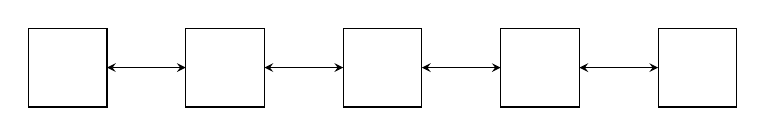
\begin{tikzpicture}
        %%%%%%%%%% Nodi %%%%%%%%%%
        \foreach \x in {0,2,...,8}
            \draw (\x,0) rectangle ++(1,1);

        %%%%%%%%% Frecce %%%%%%%%%
        \foreach \x in {1,3,...,7}
            \draw[<->,>=stealth] (\x,0.5) -- ++(1,0);
    \end{tikzpicture}
\end{center}